\chapter[Evaluating Modeling Plagiarism]{Evaluating Plagiarism Detection for Modeling Assignments}\label{sec:mde-eval}

This chapter evaluates our approach to enabling token-based plagiarism detection for modeling assignments (\contribution{2}) with datasets from real-world modeling assignments. Thus, it addresses our first evaluation goal (\gref{2}).
We thus show the feasibility of applying token-based techniques for detecting modeling plagiarism and that they provide obfuscation resilience, outperforming the state-of-the-art.
We demonstrate our approach's effectiveness in detecting plagiarism based on algorithmic, AI-based, and human obfuscation.
Our results show that our approach provides resilience against automated obfuscation attacks.
%
We implemented our approach based on JPlag~\cite{prechelt2002}. In contrast to the evaluation for code in \autoref{cha:code-eval}, JPlag is thus not the baseline, as we evaluate whether we succeeded in enabling token-based plagiarism detection for artifacts of modeling assignments.
Instead, we use the LSH-based approach of \citet{Martinez2020} as a baseline.
For our implementation based on JPlag, we used the default minimal match length of 7.
For the remainder of this chapter, we use \textit{Token-based} as the identifier for our approach.
For the LSH-based approach, we used the recommended parameters for \ac{EMF} metamodels.
We avoided any parameter tuning to ensure a fair comparison.
%
Note that this evaluation stage only includes the defense mechanism for modeling languages: model subtree reordering (MSR).
To analyze the effects of MSR, we evaluate our approach with \textit{and} without it.
%, subsequence match merging, and a combination of both. The second evaluation stage covers the mechanisms that apply to modeling languages.

Our approach demonstrates broad resilience to algorithmic obfuscation attacks, clearly distinguishing between plagiarism pairs and unrelated originals. Notably, the approach of \citet{Martinez2020} shows vulnerability for renaming-based obfuscation. For human-obfuscated plagiarism, our method consistently achieves effective separation from unrelated pairs, outperforming the approach of \citet{Martinez2020}, which struggles with detection. Against AI-obfuscated plagiarism, our method achieves high similarity scores, especially in complex plagiarism-to-plagiarism comparisons, thus outperforming \citet{Martinez2020}. We provide a replication package for replicability~\fancycite{replication-package}.

The chapter is structured as follows: First, we introduce the obfuscation attacks used for evaluation. Next, we evaluate plagiarism modeling based on algorithmic obfuscation, manual obfuscation by novice modelers, and AI-based obfuscation using ChatGPT~\cite{ChatGPT}. After that, we summarize the results. Finally, we discuss threats to validity.

\ownpublications{
    \fancycite{Saglam2024a},
    \fancycite{Saglam2023}, and
    \fancycite{Saglam2022}.
}

\section{Obfuscation Attacks}
The following discusses the obfuscation attacks used for our modeling plagiarism evaluation.
In essence, we use three automated obfuscation categories: Manual, algorithmic, and AI-based. For manual obfuscation, we use models obfuscated by novice modelers (see \autoref{sec:human-plagiarism}).
We base the algorithmic obfuscation on existing works from model clone detection~\cite{Babur2019} and model refactoring~\cite{Bettini2022, Sidhu2018, Stoerrle2015}.
Finally, for AI-based obfuscation, we used twelve different prompts, leading to various model changes.

In total, we employ six categories of obfuscation attacks to evaluate modeling plagiarism (note that each category consists of multiple obfuscation types):
%We evaluate in three stages: %, according to which our evaluation is structured into two parts.
\begin{enumerate}
\small
%[style=unboxed,leftmargin=0cm,topsep=2pt]
%\begin{enumerate}[style=unboxed,leftmargin=0cm]
\item Insertion of new model elements at random valid positions in the model.
\item Random deletion of existing model elements and their children (semantic-altering).
\item Random intra- and inter-reference reordering of model elements (semantic-preserving).
\item Renaming of random elements to pseudo-sensical names based on existing names.
\item Manual, mixed-technique obfuscation by novice modelers (semantic-preserving).
\item AI-based obfuscation via ChatGPT with mixed prompts (semantic-agnostic).
%\item[S1] Evaluation for isolated attack types.
%\item[S2] Evaluation for manual plagiarism by novice modelers.
%\item[S3] Evaluation for AI-obfuscated plagiarism by ChatGPT.
%\item[S3] Evaluation for fully AI-generated plagiarism by ChatGPT
%\end{enumerate}
\end{enumerate}
Note that attack types 1. and 4. \textit{could} be considered semantic altering due to the algorithmic and randomized nature of the obfuscation attack implementation. However, this characteristic only enhances the robustness of the evaluation results, as these attacks are considered even more effective.
As discussed in \autoref{sec:mde-intrusiveness}, defining semantic-preserving obfuscation in the context of models is not as straightforward as for code. For non-executable models without formally defined semantics, intrusiveness depends on the use case.
In the context of modeling assignments, semantic-preserving obfuscation attempts to ensure that the modified model still qualifies as a valid solution, thus maintaining the same concepts.

\textbf{Algorithmic Obfuscation:}
We evaluate the first four obfuscation attacks (\textbf{1.} to \textbf{4.}) in one evaluation stage, as they are all randomization-based algorithmic obfuscation techniques. A crucial benefit of these single-type obfuscation attacks is that they allow comparisons of which types of changes a plagiarism detection system is resilient against.

We base the algorithmic obfuscation techniques on existing works from model clone detection~\cite{Babur2019} and model refactoring~\cite{Bettini2022, Sidhu2018, Stoerrle2015} and on our observations during the experiment with novice modelers described in \autoref{sec:human-plagiarism}. There are some similarities to obfuscation in code plagiarism~\cite{Karnalim2016}, but many of the employed modifications are modeling-specific.
%
We omit trivial attacks (Type-A~\cite{Babur2019}, L0/L1~\cite{Karnalim2016}) like verbatim copying, attacks against which our approach and the LSH-based approach are inherently resilient. This includes attacks like changing the type of attributes, the multiplicity of references, and trivial name changes like typographical errors.
We also omit attacks that do not affect our approach or the one of \citet{Martinez2020}. This includes, for example, the modification of enumerations, annotations, default values, \textit{ordered} or \textit{unique} constraints, or generics.

\begin{table}[b]
	\centering
	\begin{tabular}{l c c c c c c c c}
		\toprule
		Attack & 
		\multicolumn{1}{l}{\rlap{\rotatebox{45}{\small{Package}}}} & \multicolumn{1}{l}{\rlap{\rotatebox{45}{\small{Class}}}} & \multicolumn{1}{l}{\rlap{\rotatebox{45}{\small{Operation}}}} & \multicolumn{1}{l}{\rlap{\rotatebox{45}{\small{Attribute}}}} &
		\multicolumn{1}{l}{\rlap{\rotatebox{45}{\small{Reference}}}} & \multicolumn{1}{l}{\rlap{\rotatebox{45}{\small{Supertype}}}} &
		Level  & Type \\
		\midrule
		Insert Element   & \checkmark & \checkmark & \checkmark & \checkmark & \checkmark & \checkmark & L2.5, L3, L4 & B, C \\
		Delete Element   & --         & \checkmark & --         & \checkmark & \checkmark & \checkmark & --           & B    \\
		Reorder Elements & \checkmark & \checkmark & --         & \checkmark & \checkmark & --         & L2.5, L3     & B, C \\
		Rename Element   & \checkmark & \checkmark & --         & \checkmark & \checkmark & --         & L2, L2.5     & C    \\
		\bottomrule
	\end{tabular}
    \caption[Algorithmic Obfuscation Attacks]{Algorithmic obfuscation attack types employed in this evaluation and their corresponding clone level \cite{Karnalim2016} and type \cite{Babur2019}. Adapted from \cite{Saglam2022}.}
	\label{tab:mde-algo-attacks}
\end{table}%

We executed these obfuscation techniques on different element types, for this \autoref{tab:mde-algo-attacks} gives an overview.
%We executed the modification for each attack on ten random model elements of the same type.
We chose random positions of all possible valid positions for a given element type to insert elements. 
Regarding the insertion of references and supertypes, we referenced random existing classes. Note that insertion, like introducing a new supertype, also affects references. Thus, it is not a pure insertion as in code obfuscation.
%
For deletion, we are limited to deleting existing elements in the models, which also affects potential child elements. For example, deleting a classifier also deletes all contained structural features. Note that this type of attack inherently affects the degree to which a given model correctly fulfills the assignments. However, we still included this attack for completeness.
%
We executed the reordering by moving elements to a randomly chosen position that was valid for the given element type.
This includes both moving elements across containment relations (e.g., moving classes to other packages) and reordering model elements in a single n-ary containment relation (e.g., reordering the attributes of a class). As for deletion, this might affect child elements. Moving a class involves moving all contained features as well.
%
For renaming and the names of inserted elements, we generated realistic names based on the fragments of existing names in the metamodel, which are indistinguishable at first glance. We included renaming, as the LSH-based approach by \citet{Martinez2020} uses names as part of the LSH signatures.

Due to the limited use of operations in the metamodels of our dataset, we only performed insertion for operations.
We also omitted the deletion of packages as this drastically alters the model semantically and is thus not a realistic obfuscation attack.
We also committed some more complex obfuscation types on purpose, as with increased complexity, they can be less frequently applied (see \autoref{fig:clone-types}), thus not altering the tokens sequences broadly, limiting effectiveness.


\textbf{Manual Obfuscation:}
In the second stage, we evaluate with human-made, mixed-technique obfuscation by novice modelers (\textbf{5.}).
We use the dataset introduced in \autoref{sec:human-plagiarism} for this, based on our experiment on modeling plagiarism. These plagiarism instances were created by novice modelers provided with the metamodeling assignment outlined in \autoref{sec:datasets} along with pre-existing solutions from the corresponding dataset. The participants made various changes, with an average of 43.7 changes per participant and a median of 31.5. On average, this corresponds to one change for every two model elements.

Participants frequently performed renaming operations, such as modifying element names or altering their formatting, to obfuscate the model while preserving its structure. Reordering elements within packages or models was another common approach, leveraging the flexibility in the order of multi-valued references. Structural modifications, such as introducing or dissolving packages, altering properties like cardinalities, and inserting and deleting features or classifiers, were also widely used. For details, please refer to \autoref{tab:student-obfuscation}.
%These obfuscation types align with the algorithmic obfuscation in the previous evaluation stage.

\textbf{AI-based Obfuscation:}
Finally, we used plagiarism instances created via AI-based obfuscation with ChatGPT for the last stage (\textbf{6.}). 
As discussed in \autoref{sec:ai-plagiarism}, we investigated fully-generating solutions with ChatGPT. However, since this produced invalid and obviously suspicious models due to the currently limited modeling capabilities of ChatGPT~\cite{Camara2023}, we chose solutions obfuscated by ChatGPT to evaluate our approach and compare it with the state-of-the-art.
Note that this evaluation was done with ChatGPT 3.5, which was, at the time, the most recent available version.
%
We used ChatGPT to generate obfuscated versions of models from the base dataset introduced in \autoref{sec:datasets}.
This method requires little modeling knowledge and produces plagiarism that is well obfuscated and relatively inconspicuous to the human eye.
While using ChatGPT occasionally led to minor syntactical issues, we mainly produced correct models that were obfuscated according to our instructions.
As discussed in \autoref{subsec:chatgpt-obf}, we provided ChatGPT with models from the dataset and applied twelve different prompts for two models to generate a total of 24 plagiarism instances.

Interestingly, the produced modifications are diverse but, more importantly, modeling-specific.
They involved various modifications to the modeling artifacts, altering their structure while maintaining plausibility within the assignment domain. These changes included adding, deleting, restructuring, and reordering elements. Moreover, this involved the manipulation of containment and supertype hierarchies. We observed restructuring models by introducing new superclasses and moving elements into these new classes. Names were altered using abbreviations, synonyms, or domain-specific prefixes and suffixes, while properties like multiplicities were adjusted. Additionally, some changes included the addition of new domain-relevant structures, such as creating a \texttt{Node} class with relationships to existing classes like \texttt{Link} and \texttt{Container}, or deduplicating attributes by introducing abstract superclasses like \texttt{NamedElement}.
%
Most of these transformations appeared natural and plausible, fitting into the context of the assignment. Even when inconsistencies or issues arose, they resembled typical human errors. However, few modifications stood out due to illogical naming conventions or less coherent structural changes.

\section{Algorithmic Obfuscation}

\label{subsec:first-stage}

\noindent
Our first stage demonstrates broad resilience to different types of algorithmic obfuscation attacks.
As discussed, we evaluate the insertion, deletion, rendering, and renaming of model elements.
There, we applied each obfuscation attack 20 times to a randomly chosen human-made model.
In total, four original metamodels were chosen, thus generating 80 plagiarism instances.
This stage is particularly useful to determine how different approaches perform for singular attack types. 

\begin{figure}
\centering
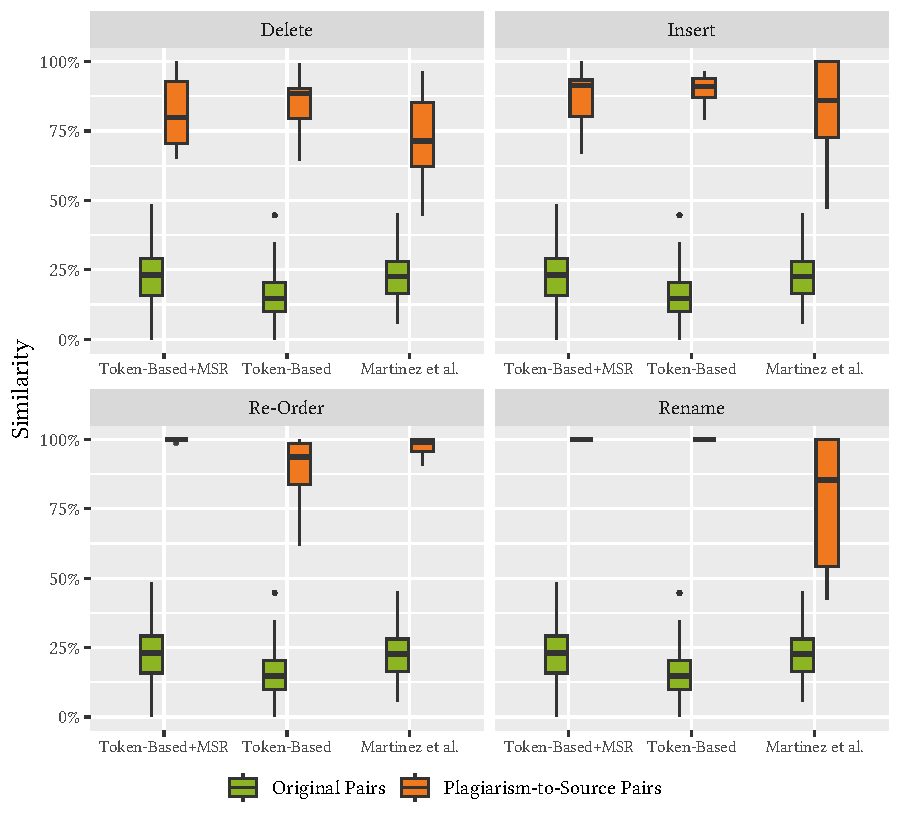
\includegraphics[width=1\linewidth]{figures/disseval2/attacktypes_avg.similarity.pdf}
\caption[Evaluation: Algorithmic Obfuscation of Models]{Results for the attack type evaluation for our token-based approach (Token-Based) with and without MSR and the LSH-based approach by \citet{Martinez2020}.}
\label{fig:attacktypes-results}
\end{figure}


 \subsection{Results}
\autoref{fig:attacktypes-results} shows the results for the different attack types.
% DELETION
For deletion attacks, all approaches can be affected by deleting elements and their children. However, this effect is limited for our approaches, as only few plagiarism instances drop below a similarity of 75\% to their source metamodels. Notably, its effect is larger with MSR enabled.
In contrast, for the LSH-based approach of \citet{Martinez2020}, this is the case for more than half of the plagiarism-to-source pairs. The median value drops below 75\%.
% INSERTION
In contrast to deletion attacks, all approaches are only slightly affected by insertion. Our approaches perform very well, achieving median similarity values above 90\%. The approach of \citet{Martinez2020} performs slightly worse but still maintains a high median value.
However, for insertions and deletions, their approach has some outliers that come close to the similarity values of the original pairs.
% MOVE
For Reordering-based attacks, the approach of \citet{Martinez2020} also performs well, showing little effect of the obfuscation attack.
Our variant without MSR, however, can be affected by reordering attacks, showing only some resilience.
In contrast, with MSR enabled, our approach shows little to no effect on the obfuscation attack. This shows that MSR makes the detection virtually invariant to reordering, thus fulfilling its purpose.
% MOVE
For renaming-based obfuscation attacks, our approaches show complete immunity, which is an inherent trait of token-based approaches.
In contrast, the approach of \citet{Martinez2020} is prone to renaming, showing a $Q_1$ at around 55\%, thus having many pairs close to the unrelated originals. This shows the advantage of token-based approaches.

\begin{table}[b]
	\centering
    \small
	\begin{tabular}{llrrr}
		\toprule
		Obfuscation Type                            & Approach        & $\Delta$ Mean & $\Delta$ Median & $\Delta$ IQR  \\
		\midrule
		\multirow{3}{*}{Delete}                     & Token-Based + MSR     & 60.21  & 59.24    & 42.86 \\
		                                            & Token-Based           & \B{72.28}  & \B{74.01}    & \B{61.90} \\
		                                            & Martinez et al. & 50.14  & 48.72    & 33.98 \\
        \midrule
		\multirow{3}{*}{Insert}                     & Token-Based + MSR     & 65.74  & 68.69    & 51.81 \\
		                                            & Token-Based           & \B{76.32}  & \B{77.05}    & \B{67.60} \\
		                                            & Martinez et al. & 60.74  & 63.28    & 44.43 \\
        \midrule
		\multirow{3}{*}{Re-Order}                   & Token-Based + MSR     & \B{76.09}  & 76.47    & \B{69.77} \\
		                                            & Token-Based           & 73.79  & \B{77.95}    & 62.20 \\
		                                            & Martinez et al. & 75.41  & 76.30    & 67.63 \\
        \midrule
		\multirow{3}{*}{Rename}                     & Token-Based + MSR     & 76.14  & 76.47    & 69.77\\
		                                            & Token-Based           & \B{84.04}  & \B{84.29}    & \B{78.45} \\
		                                            & Martinez et al. & 55.49  & 62.72    & 26.16 \\
		\bottomrule
	\end{tabular}
    \caption[Evaluation: Algorithmic Obfuscation of Models]{Similarity differences between the algorithmically obfuscated plagiarism instances and the unrelated originals (higher means better detection) for the results in \autoref{fig:attacktypes-results}.}
	\label{tab:summary-stats-algo}
\end{table}


\subsection{Discussion}
Note that with limited obfuscation strength, the effects of the normalization are less pronounced, and thus, when looking at the similarity differences (\autoref{tab:summary-stats-algo}), our approach without MSR performs quite well, as our approach with MSR has smaller differences due to the increase for original pairs. As we use a singular obfuscation type with limited modifications in this stage, the possible effects of the normalization are inherently limited.

While deletion-based attacks seem effective on paper, they are not feasible in practice.
Usually, very little can be removed from an assignment's artifact without making the solution incomplete or even plain wrong.
In our evaluation, we randomly removed elements along with their children, which sometimes resulted in removing large subtrees (thus explaining why its effect is slightly stronger with MSR enabled). With that in mind, the effects of these attacks were relatively mild, and our approach still allows differentiation between plagiarism pairs and original pairs. However, the approach of \citet{Martinez2020} is more affected by deletion attacks.

Regarding insertion attacks, our approach shows resilience, while for renaming, our approach demonstrates complete immunity. Without MSR, our approach is prone to reordering-based attacks, which motivates the need for MSR. In contrast, the approach from \citet{Martinez2020} is strongly vulnerable to renaming-based attacks but not vulnerable to reordering attacks.
It is worth noting that renaming and reordering are probably the most trivial attacks, both for humans and computers~\cite{Saglam2023}.

\textit{Overall, our approach performs well, outperforming the approach of \citet{Martinez2020}, which is considered the state of the art.}


% -------------------------
% Eval Stage 2
% -------------------------

\section{Manual Obfuscation by Novice Modelers}

\begin{figure}[b]
\centering
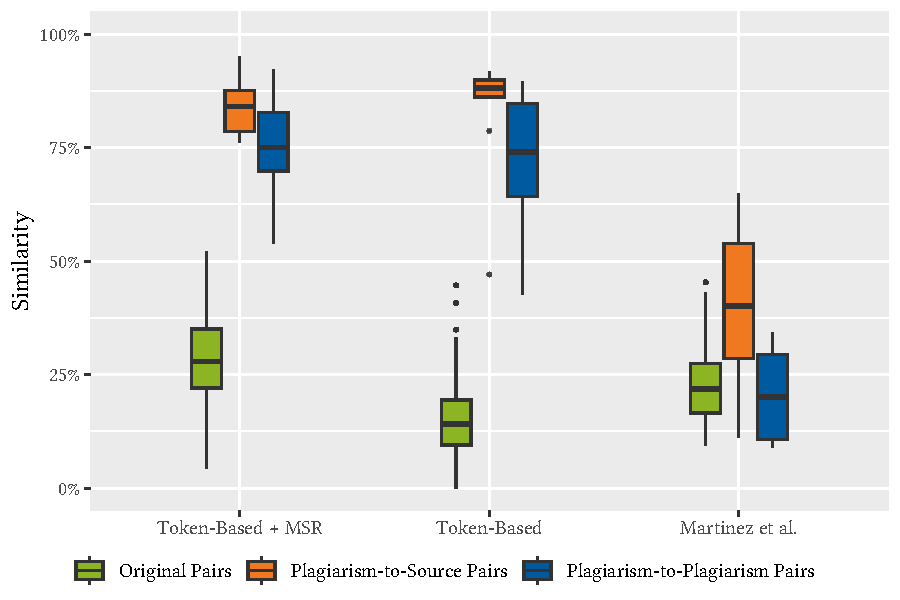
\includegraphics[width=1\linewidth]{figures/disseval2/experiment_avg.similarity.pdf}
\caption[Evaluation: Human Obfuscation of Models]{Results regarding human-generated plagiarism for our token-based approach (Token-Based) with and without MSR and the LSH-based approach by \citet{Martinez2020}.}
\label{fig:human-results}
\end{figure}

\noindent
The second stage evaluates based on instances of human-obfuscated plagiarism by novice modelers.
Note that these obfuscation attempts were the weakest in our overall evaluations. This motivates why automated obfuscation is a viable alternative for a potential adversary.

As discussed, we use our modeling plagiarism experiment dataset introduced in \autoref{sec:human-plagiarism} for this.
It consists of 31 metamodels, thus producing 210 unrelated, original pairs, ten plagiarism-to-source, and ten indirect plagiarism-to-plagiarism pairs (pairs of plagiarized models of the same source). Refer to \autoref{tab:student-obfuscation} for details on the employed obfuscation techniques.

\subsection{Results}
The results of the manually obfuscated plagiarism by novice modelers are illustrated in \autoref{fig:human-results}.
The results demonstrate that with MSR enabled, our approach can effectively distinguish the plagiarism-to-source pairs from the unrelated original pairs, as there is no overlap. Without MSR, our approach demonstrates good separation except for one outlier falling below 50 percent similarity. However, for the approach of \citet{Martinez2020}, the plagiarism-to-source pairs still exhibit increased similarities but overlap with the unrelated pairs, making detection more challenging.
When looking at the similarity differences in \autoref{tab:summary-stats-human}, we notice that the similarity differences are higher for our approach when MSR is disabled.
%
Similar results are observed for the plagiarism-to-plagiarism pairs. With MSR, our approach exhibits a clear separation between plagiarism pairs and unrelated pairs. Without it, there is sufficient separation between them, although a few outliers overlap with the unrelated pairs at around 40 percent similarity. In contrast, for \citet{Martinez2020}, the plagiarism-to-plagiarism median similarity falls below the median of the unrelated pairs, making detection next to impossible.
Again, when looking at the similarity differences, we notice that the similarity differences are higher for our approach when MSR is disabled.

\begin{table}%[h]
	\centering
	\begin{tabular}{llrrr}
		\toprule
		Plagiarism Type                             & Approach        & $\Delta$ Mean & $\Delta$ Median & $\Delta$ IQR  \\
		\midrule
		\multirow{3}{*}{Plagiarism-to-Source}       & Token-Based + MSR     & 55.47  & 55.40    & 43.79 \\
		                                            & Token-Based           & \B{69.19}  & \B{74.48}    & \B{65.57} \\
		                                            & Martinez et al. & 16.78  & 18.30    & 1.10 \\
        \midrule
		\multirow{3}{*}{Plagiarism-to-Plagiarism}   & Token-Based + MSR     & 46.36  & 46.55    & 33.25 \\
		                                            & Token-Based           & \B{57.03}  & \B{62.68}   & \B{43.74} \\
		                                              & Martinez et al. & -2.12  & -1.70    & -16.68 \\
		\bottomrule
	\end{tabular}
    \caption[Evaluation: Human Obfuscation of Models]{Similarity differences between the manually obfuscated plagiarism instances and the unrelated originals (higher means better detection) for the results in \autoref{fig:human-results}.}
	\label{tab:summary-stats-human}
\end{table}



\subsection{Discussion}
Some instances of manual plagiarism were sufficiently well-obfuscated to yield low similarities for our approach without MSR~\cite{Saglam2022}.
These instances accomplished this by heavily relying on reordering model elements, which is the vulnerability that MSR aims to address.
This observation aligns with the results of the first evaluation stage depicted in \autoref{fig:attacktypes-results}. MSR is explicitly designed to address this type of attack.
%
Nevertheless, both with and without MSR, our approach yields overall high similarities for plagiarism-to-source pairs.
We observed relatively weak obfuscation for these plagiarism pairs. The manual obfuscation observed here is thus weaker than automated obfuscation attacks.
Due to this weak obfuscation, MSR's effect is limited in many of the comparisons. However, it still notably improves the detection of outliers. 
We can observe a more noticeable impact of MSR for the plagiarism-to-plagiarism pairs, where the difference between the compared models is more pronounced, as it reflects the obfuscation efforts of two students instead of one.
%
Overall, our approach without MSR exhibits a lower similarity for the unrelated pairs, which can be attributed to our normalization technique.
The normalization reduces the impact of certain structural and syntactic variations between the unrelated pairs, thus slightly increasing their similarity.
This effect, however, does not impact the separability of the original from the plagiarism pairs.
In fact, the distinction between the stronger obfuscated instances and the original pairs is considerably more pronounced with MSR enabled than with it disabled.

\emph{In sum, our approach demonstrates strong performance in detecting human plagiarism, whereas the approach of \citet{Martinez2020} performs worse.}


% -------------------------
% Eval Stage 3
% -------------------------

\section{AI-based Obfuscation}\label{subsubsec:plaggpt}

\noindent
In our third and main evaluation stage, we evaluate the ability to detect comprehensively AI-obfuscated plagiarism.
%
As discussed in \autoref{subsec:chatgpt-obf}, we provided ChatGPT with models from the dataset and applied twelve different prompts for two metamodels to generate a total of 24 plagiarism instances. To evaluate the effects of even stronger obfuscation, we do not only evaluate with the plagiarism-to-source pairs but also with the pairs of plagiarized models of the same source (plagiarism-to-plagiarism, see \autoref{sec:metrics}).
Thus, we evaluate 24 Plagiarism-to-Source pairs and 132 Plagiarism-to-plagiarism pairs, which must be distinguished from the 210 unrelated original pairs (true negatives).

\subsection{Results}

\noindent
\autoref{fig:ai-obfuscated-models} shows the results for plagiarism generated by ChatGPT.
For the plagiarism-to-source pairs, our approach achieves high median scores of 78\% (MSR) and 74\% (no MSR), respectively. The approach of \citet{Martinez2020} has a significantly lower median score of 59\%. We observe similar results when looking at the difference between the plagiarism-to-source pairs and the unrelated original pairs as listed in \autoref{tab:summary-stats}. Our approach achieves the highest values for all three similarity \textit{difference} metrics ($\Delta$ Mean, $\Delta$ Median, and $\Delta$ IQR). Our approach without MSR follows closely by between three to five percentage points. The approach of \citet{Martinez2020} performs significantly worse, with 17 to 25 percentage points below our approach.

The differences between the approaches are even more prominent when looking at the similarity scores of the plagiarism-to-plagiarism pairs.
Our approach achieves a median score of 67\% with MSR enabled, 53\% without MSR, and \citet{Martinez2020} achieve only 43\%.
Our approach with MSR achieves the highest values for the difference between the plagiarism-to-plagiarism pairs and the unrelated original pairs listed in \autoref{tab:summary-stats}.
Without MSR, it achieves between eight to twelve percentage points less, \citet{Martinez2020} achieves between 21 to 25 percentage points less.

To determine the statistical significance of the evaluation results presented in \autoref{fig:ai-obfuscated-models}, we conducted one-sided Wilcoxon rank-sum tests with a significance level of $\alpha=0.05$. Ideally, to demonstrate a significantly improved performance, an approach has to show significantly higher scores for the plagiarism pairs (P2S and P2P) and significantly lower scores for the unrelated original pairs (OP). We both test for the effect of MSR and for the improvement of our approach with MSR compared to the approach of \citet{Martinez2020}. The results of the tests are summarized in Table \ref{tab:significance-stats}.
As the test statistic value ($W$) depends on the sample size and the sample sizes of the pair types differ, we use Cliff's delta ($\delta$) as a normalized metric for the effect size.

In the context of the Plagiarism-to-Source (P2S) and Plagiarism-to-Plagiarism (P2P) pairs, MSR significantly improved the similarity scores.
Furthermore, our approach performs significantly better than the approach of \citet{Martinez2020}.
While our approach with MSR achieves significantly lower scores for the original pairs (OP) compared to \citet{Martinez2020}, this is not the case for our approach without MSR.
However, the (negative) effect size of the original pairs is smaller than the effect sizes for the plagiarism pairs, which aligns with the similarity score differences in \autoref{tab:summary-stats}. As a consequence, this shift is negligible.
In summary, we observe both statistical and practical significance for the improvements brought by MSR and for the improvements of our approach (with MSR) compared to the one of \citet{Martinez2020}.

\begin{figure}
    \centering
    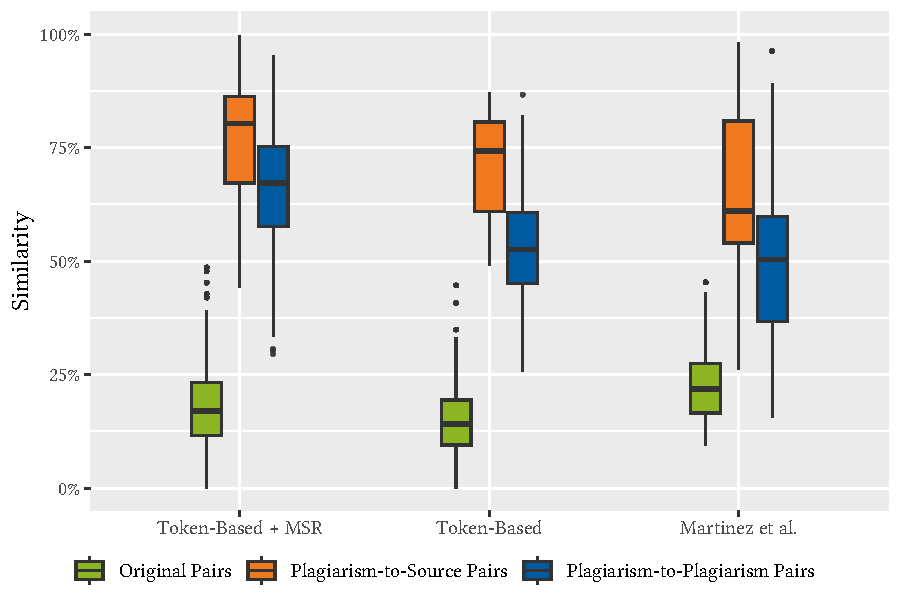
\includegraphics[width=\linewidth]{figures/disseval2/chatgpt_avg.similarity.pdf}
    \caption[Evaluation: AI-based Obfuscation of Models]{Results regarding ChatGPT-obfuscated plagiarism for our token-based approach (Token-Based) with and without MSR and the LSH-based approach by \citet{Martinez2020}.}
    \label{fig:ai-obfuscated-models}
\end{figure}

 \subsection{Discussion}
Our evaluation found that our approach significantly outperforms the state-of-the-art regarding the detection of AI-obfuscated models.
This is especially apparent when the obfuscation is strong, which is true for plagiarism-to-plagiarism pairs.
While our approach with MSR disabled also performs well, it is less resilient to strong obfuscation attempts.
This can be attributed to it being susceptible to reordering attacks, as shown in \autoref{subsec:first-stage}.
However, with MSR enabled, it is resilient to these attacks due to the benefits of this normalization technique.
Reordering and renaming are also likely the first steps a potential adversary would take after utilizing ChatGPT~\cite{Saglam2023}. 

The difference between our approach and \citet{Martinez2020} is even more considerable, as ChatGPT frequently employs renaming.
The renaming attacks of ChatGPT are particularly effective, as ChatGPT considers the modeling domain and identifies suitable synonyms.
Interestingly, as ChatGPT is partially deterministic, we observed recurring patterns for different prompts, such as inserting a \enquote{Node} and \enquote{Edge} class and adding references from specific existing classes to the inserted one. This shows that even with systematic prompt engineering and strong obfuscation, plagiarizers cannot be certain to avoid detection.

\emph{In sum, plagiarism generated with ChatGPT currently is predictable enough to be reliably detected by our approach. Our approach also significantly outperforms the state-of-the-art, especially for strongly obfuscated plagiarism.}

\begin{table}%[h]
	\centering
	\begin{tabular}{llrrr}
		\toprule
		Plagiarism Type                                             & Approach        & $\Delta$ Mean & $\Delta$ Median & $\Delta$ IQR  \\
		\midrule
		\multirow{3}{*}{Plagiarism-to-Source}                       & Token-Based + MSR            & \B{59.77}  & \B{64.39}    & \B{45.37} \\
		                                                            & Token-Based   & 56.87  & 60.22    & 40.23 \\
		                                                            & Martinez et al. & 42.16  & 39.27    & 26.54 \\
        \midrule
		\multirow{3}{*}{Plagiarism-to-Plagiarism}                   & Token-Based + MSR            & \B{48.01}  & \B{50.94}    & \B{33.80} \\
		                                                            & Token-Based   & 39.12  & 38.56   & 25.64 \\
		                                                            & Martinez et al. & 27.43  & 28.58    & 9.20 \\
		\bottomrule
	\end{tabular}
    \caption[Evaluation: AI-based Obfuscation of Models]{Similarity differences between the AI-based plagiarism instances and the unrelated originals (higher means better detection) for the results in \autoref{fig:ai-obfuscated-models}.}
	\label{tab:summary-stats}
\end{table}

\begin{table}%[h]
	\centering
	\begin{tabular}{lllrrrr}
		\toprule
		Comparison                                                  & Pairs & $H1$  & $p$         & $W$     & $\delta$ &   $n$  \\
		\midrule
		\multirow{3}{*}{Effects of Normalization}           & P2S & greater &  0.042  & 373     & 0.293         & 24         \\
		                                                              & P2P & greater & <0.001  & 13,024  & 0.495         & 132       \\
		                                                              & OP  & less    & 1.000   & 232,839 & 0.173         & 630    \\
		\midrule
		\multirow{3}{*}{{Token-Based + MSR to Martinez}}                  & P2S & greater & 0.008   & 405     & 0.406         & 24        \\
		                                                              & P2P & greater & <0.001  & 13,291  & 0.526         & 132        \\
		                                                              & OP  & less    & <0.001  & 131,810 & -0.336        & 630     \\
		\bottomrule
	\end{tabular}
    \caption[Significance: AI-based Obfuscation of Models]{Significance of the results in \autoref{fig:ai-obfuscated-models} assessed via one-sided Wilcoxon rank-sum tests (sign. level of $\alpha=0.05$, alternative hypothesis $H1$, p-value $p$, test statistic $W$, Cliff's delta $\delta$, sample size $n$) for Plagiarism-to-Source (P2S), Plagiarism-to-Plagiarism (P2P), and Original Pairs (OP).}
    \label{tab:significance-stats}
\end{table}

\section{Result Summary}\label{sec:mde-result-summary}
Our approach for token-based plagiarism detection for modeling assignments demonstrates broad resilience to algorithmic obfuscation attacks.
Notably, the approach of \citet{Martinez2020} shows vulnerability for renaming-based obfuscation, for which token-based approaches are inherently immune against.
For human-obfuscated plagiarism, our approach outperforms the approach of \citet{Martinez2020}, which encounters difficulties in detection.
Against AI-obfuscated plagiarism, our method achieves high similarity scores, especially in the strongly obfuscated plagiarism-to-plagiarism comparisons, thus outperforming \citet{Martinez2020} by a significant margin. The statistical tests further confirm the statistical and practical significance of these results.

Based on these results, we can answer the evaluation questions as follows:
\summaryBox{2.1}{Token-based detection approaches can successfully be applied to artifacts of modeling approaches, thus allowing for efficient and effective plagiarism detection.}
\summaryBox{2.2}{Token-based plagiarism detection significantly outperforms state-of-the-art modeling plagiarism detection when applied to modeling artifacts.}
\summaryBox{2.3}{Our token-based approach inherits the inherent immunity to renaming-based obfuscation but also achieves broad resilience against various human, algorithmic, and AI-based obfuscation attacks.}

In conclusion, we have achieved our evaluation goal \textbf{G2} of enabling token-based plagiarism detection for modeling assignments, providing a robust framework for identifying and addressing instances of plagiarism in this domain.

\section{Threats to Validity}
We now discuss how we address threats to the validity of our evaluation, following the guidelines outlined by \citet{Wohlin2012} and \citet{runeson2008}. These threats apply to the second goal of our evaluation, which aims to enable token-based plagiarism detection for artifacts of modeling assignments (\gref{2}).


\subsection{Internal Validity}
Internal validity refers to whether influences can unknowingly affect the analyzed variable concerning causality~\cite{Wohlin2012}.

    \textbf{Baseline Consistency:} For internal validity, we used the LSH-based approach of \citet{Martinez2020} as it is state-of-the-art. Besides this, we ensured that all other conditions remained constant when comparing the defense mechanism with each other or with the baseline. 

    \textbf{Baseline Parametrization:} As the approach of \citet{Martinez2020} is LSH-based, it provides several hyperparameters that may need to be adjusted to the modeling domain to maximize the detection rate. In detail, this involves the number of bands, which affects the strictness of the signature matching, and the number of rows per band, which controls the trade between precision and recall. This threatens internal validity, as incorrect or non-optimized parameter settings could affect the outcome~\cite{novak2018}. To mitigate this, we used the recommended parameters for \ac{EMF} metamodels discussed by the authors.

    \textbf{Human-Labeled Plagiarism}: If any datasets are manually labeled plagiarized, evaluator bias could influence these labels.
    However, this threat does not apply to our evaluation, as we can provide inherently correct labels for all plagiarism types.
    We generate the plagiarism instances for the automatic obfuscation, thus knowing which models are plagiarized.
    For human plagiarism, we obtained these by conducting a controlled experiment (see \autoref{sec:human-plagiarism}).

\subsection{External Validity}
External validity concerns the extent to which our findings can be generalized beyond the specific context of the evaluation. 

    \textbf{Availability of Datasets:} One potential limitation is the scarcity of publicly available modeling assignments datasets. Due to privacy and data protection policies, students' data is rarely published. For modeling plagiarism, we mitigated this by designing our evaluation around the widely used EMF-based metamodels, using a representative dataset from a real-world assignment~\cite{Saglam2023}.
    We thus transform it into three different data sets using various types of plagiarism (algorithmic, AI-based, and human).
    EMF-based metamodels are widely-used, and metamodeling is a typical assignment~\cite{Ciccozzi2018}.
    We acknowledge that additional datasets could provide further validation, yet the selected dataset and tasks reflect standard practices in educational settings.


    \textbf{Prompt Choice:} For AI-based obfuscation with ChatGPT, prompt choice is an essential factor influencing the strength and variability of AI-generated plagiarism. To control this, we conducted a pre-study in which we experimented with multiple prompts, incrementally adjusting them to increase the degree of obfuscation. By refining our prompts iteratively, we aimed to obtain representative results for AI-generated obfuscation effects while minimizing prompt variability as a confounding factor.

    \textbf{Generalizability of obfuscation attacks:}
    Limiting the evaluation to only a few types of obfuscation attacks could hinder the applicability of our results to broader contexts. To enhance external validity and thus ensure that our findings are generalizable, we included a diverse set of obfuscation techniques from the categories outlined in our threat model (see \autoref{sec:threatmodel-categorization}). Note that these are real-world obfuscation attacks that are, directly or conceptually, available in practice.

\subsection{Construct Validity}
Construct validity refers to how well the evaluation measures its intended purpose and whether the metrics and baselines chosen are appropriate. Thus, it relates to the degree to which we measure the theoretical construct we want to measure.

    \textbf{Evaluation Methodology Alignment:} To enhance construct validity, we aligned our evaluation methodology with those from established and related work. While we deviate from related works by not using a threshold-based classification, we do so to improve internal validity (see \autoref{sec:metrics}), as this method is fundamentally flawed. Finally, we employ an approach-independent ground truth, use established similarity metrics, and a Goal-Question-Metric plan~\cite{Basili1984, Basili1992}.

    \textbf{Underlying Research Object:} We ensure consistency between the research objects and the measurements via direct alignment. Since our study evaluates the effectiveness of modeling plagiarism detection, we use the similarity scores generated by the detectors as our primary measurement. Additionally, we directly utilize widely available techniques such as ChatGPT to assess automated obfuscation accurately.

    \textbf{Choice of Baseline:} The baseline selection might affect the comparison and outcomes. We addressed this by selecting the approach of \citet{Martinez2020} as the baseline, as it is, to our knowledge, the only other approach for plagiarism detection for modeling assignments.

\subsection{Reliability}
Reliability concerns the consistency of the results and whether the study can be replicated under the same conditions.


    \textbf{Replicability:} To ensure reliability, we provide a comprehensive replication package for our evaluation~\fancycite{replication-package}.

    \textbf{Use of Internal Datasets:} Using internal datasets can hinder reproducibility. Due to data sensitivity, only a partial dataset version is publicly available. We discussed any preprocessing steps and the employed obfuscation attacks for all datasets. Furthermore, we provide raw result data and metadata in our replication package. This enables researchers to replicate our experiments on other datasets, maintaining transparency and reliability.

%\todo{(LOW) Regarding \citet{Martinez2020}: Bad results for human plagiarism, however, may be a parameterization issue, as this approach relies heavily on that. We used the recommended parametrization for EMF metamodels, not further parameter tuning. For our approach, we also did no tuning and used default parameters.}
